\subsection{Reaction Networks}
\begin{figure}[H]
    \begin{minipage}[t][6cm][t]{.18\textwidth}
        \centering
        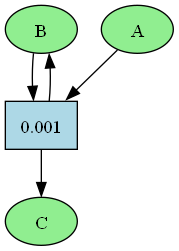
\includegraphics[width=\linewidth]{networks/simple.png}
        \caption{Reaction network for the simple model.}
        \label{fig:network_simple}
    \end{minipage}\hfill
    \begin{minipage}[t][6cm][t]{.38\textwidth}
        \centering
        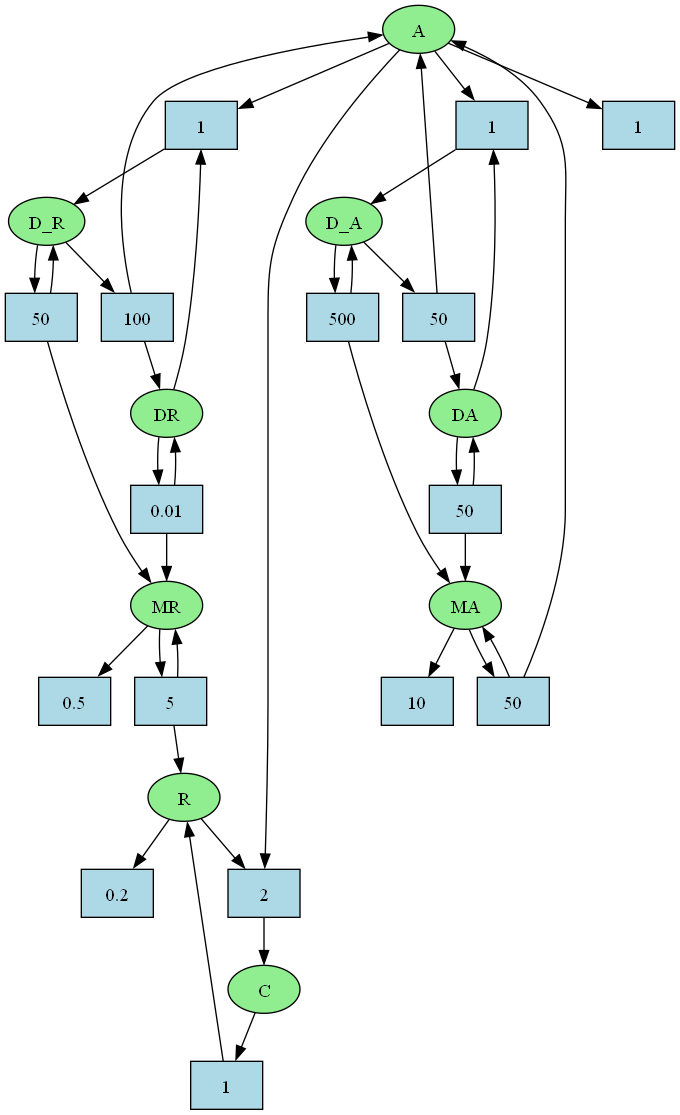
\includegraphics[width=\linewidth]{networks/circadianOscillator.png}
        \caption{Reaction network for the circadian oscillator model.}
        \label{fig:network_circadianOscillator}
    \end{minipage}\hfill
    \begin{minipage}[t][6cm][t]{.38\textwidth}
        \centering
        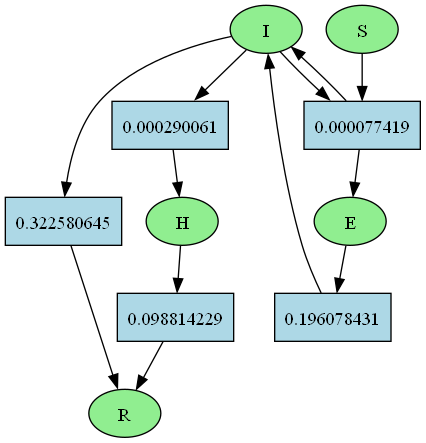
\includegraphics[width=\linewidth]{networks/seihr.png}
        \caption{Reaction network for the SEIHR model.}
        \label{fig:network_seihr}
    \end{minipage}
\end{figure}

\subsection{Plots}
\begin{figure}[H]
	\centering
	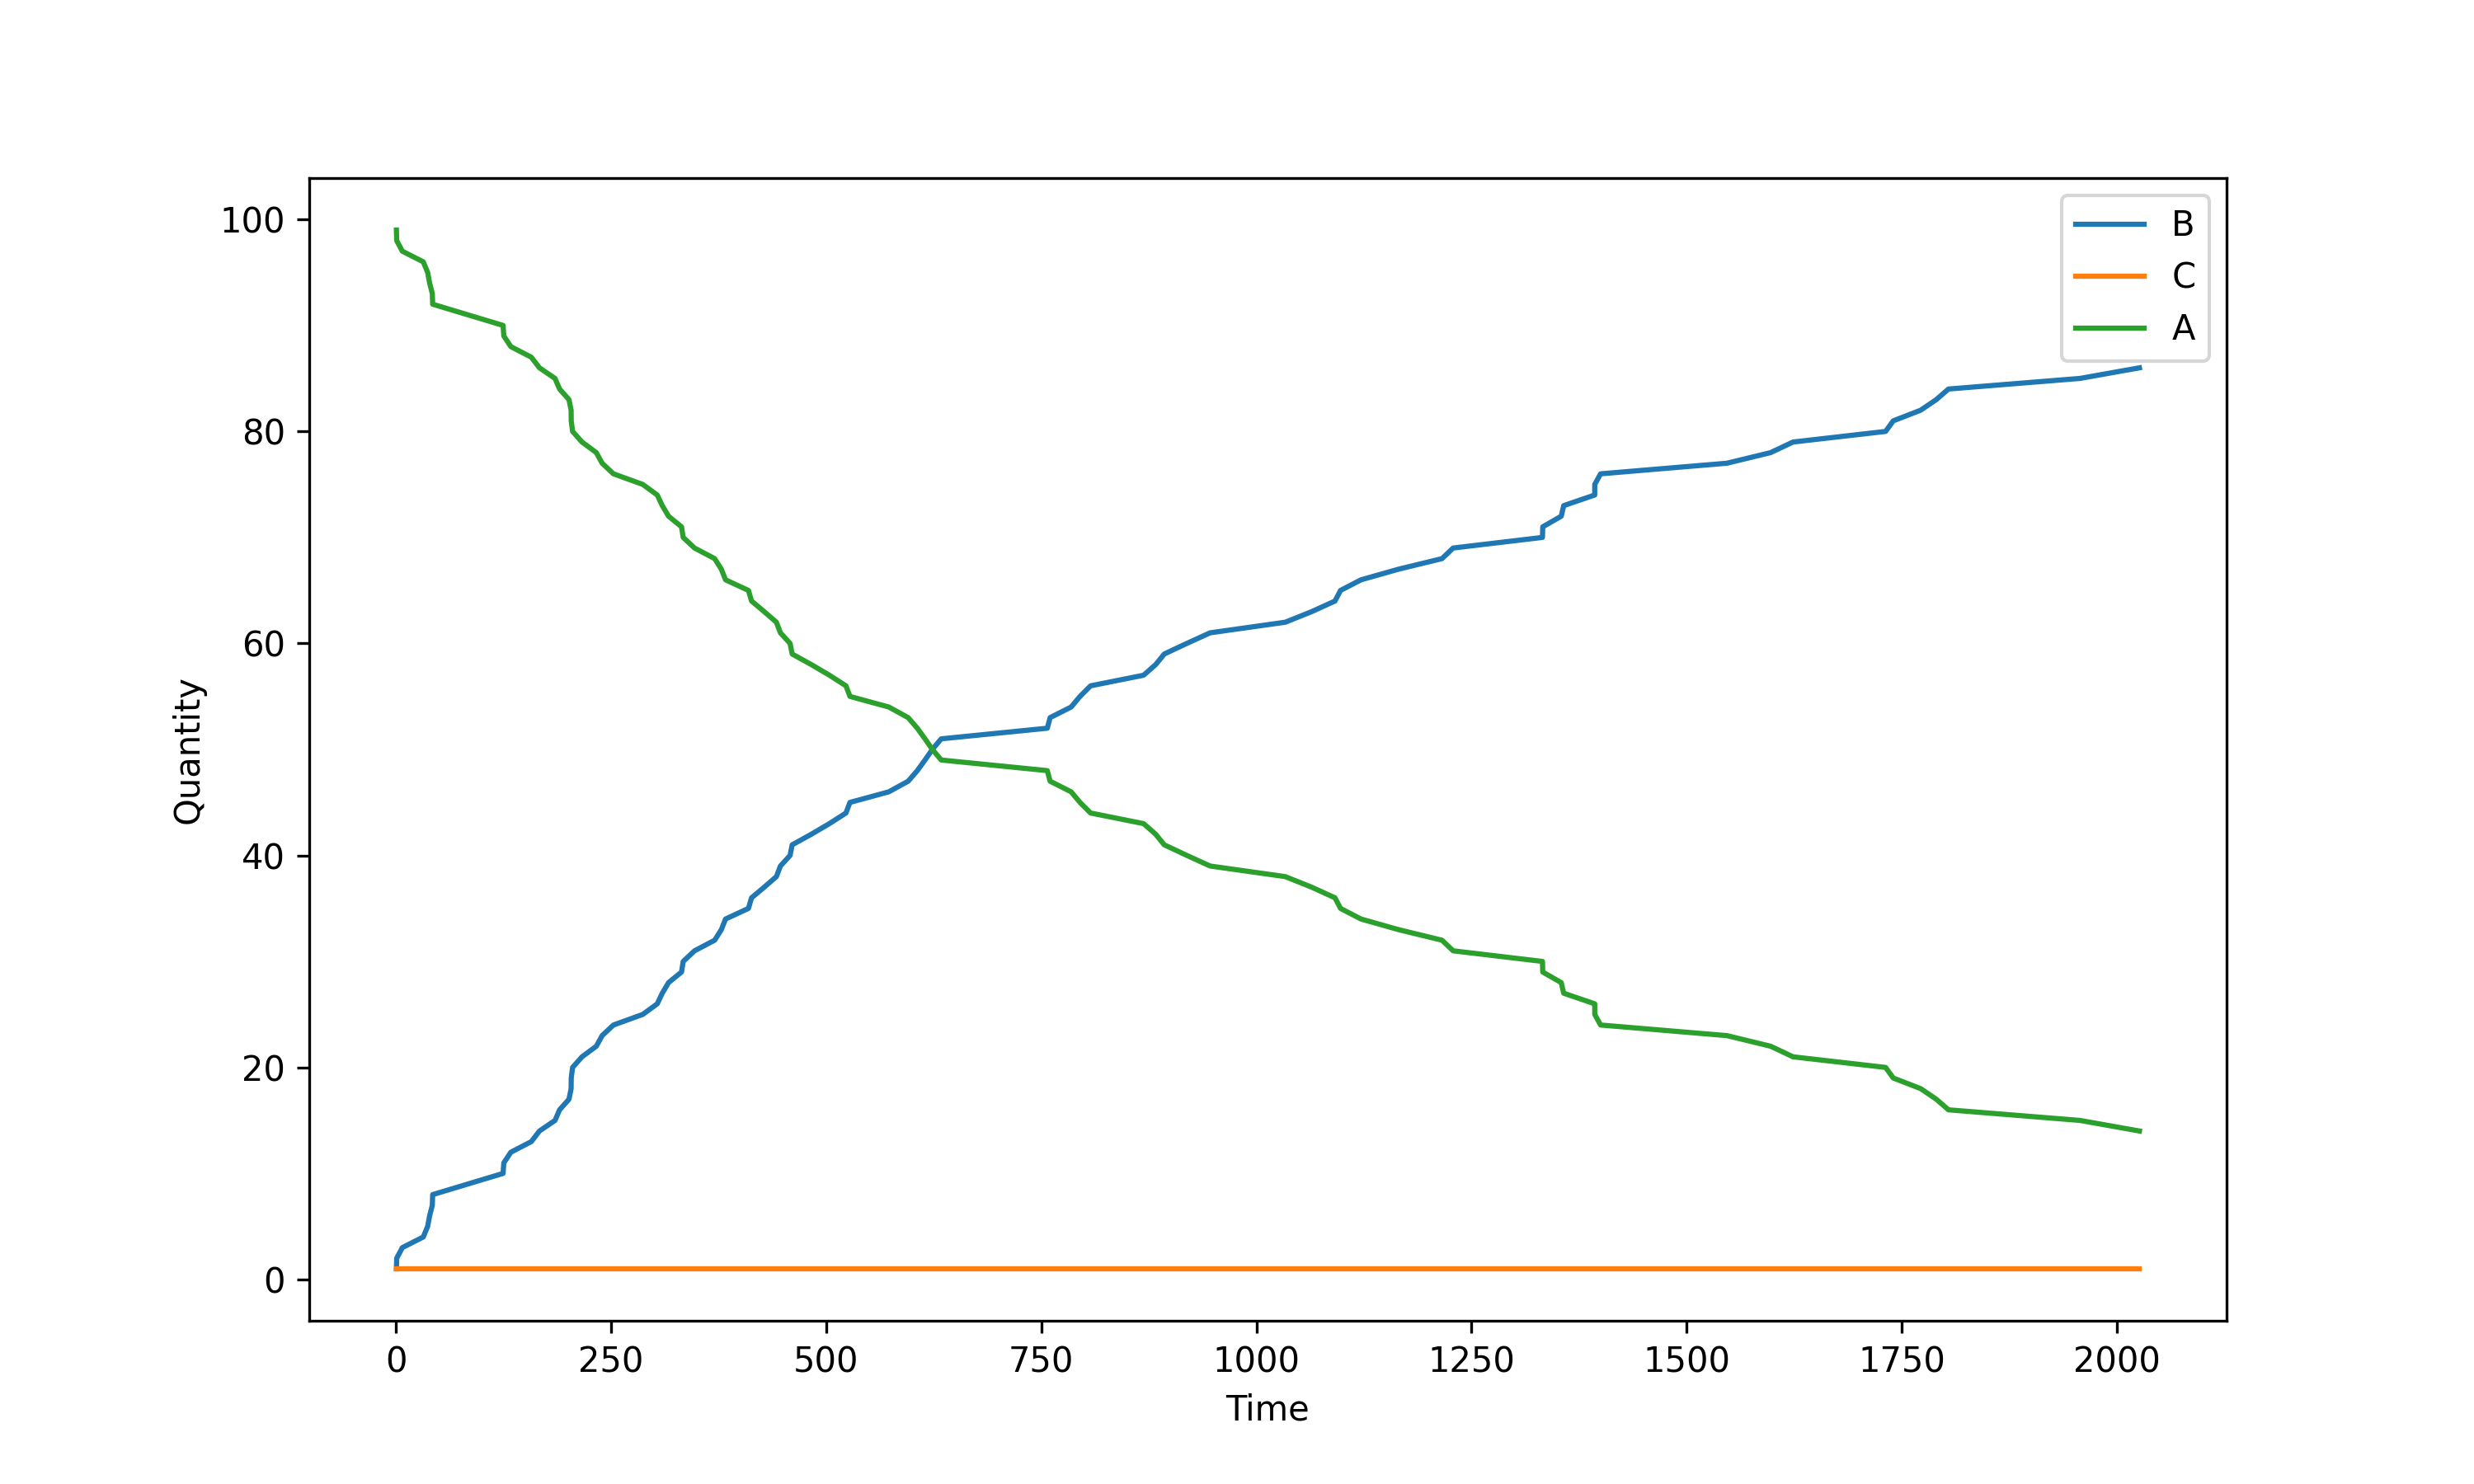
\includegraphics[width=\textwidth]{../plots/simple1}
	\caption{Plot of running the simple model simulation with A(0)=100, B(0)=0, C(0)=1.}
	\label{fig:plot_simple1}
\end{figure}

\begin{figure}[H]
	\centering
	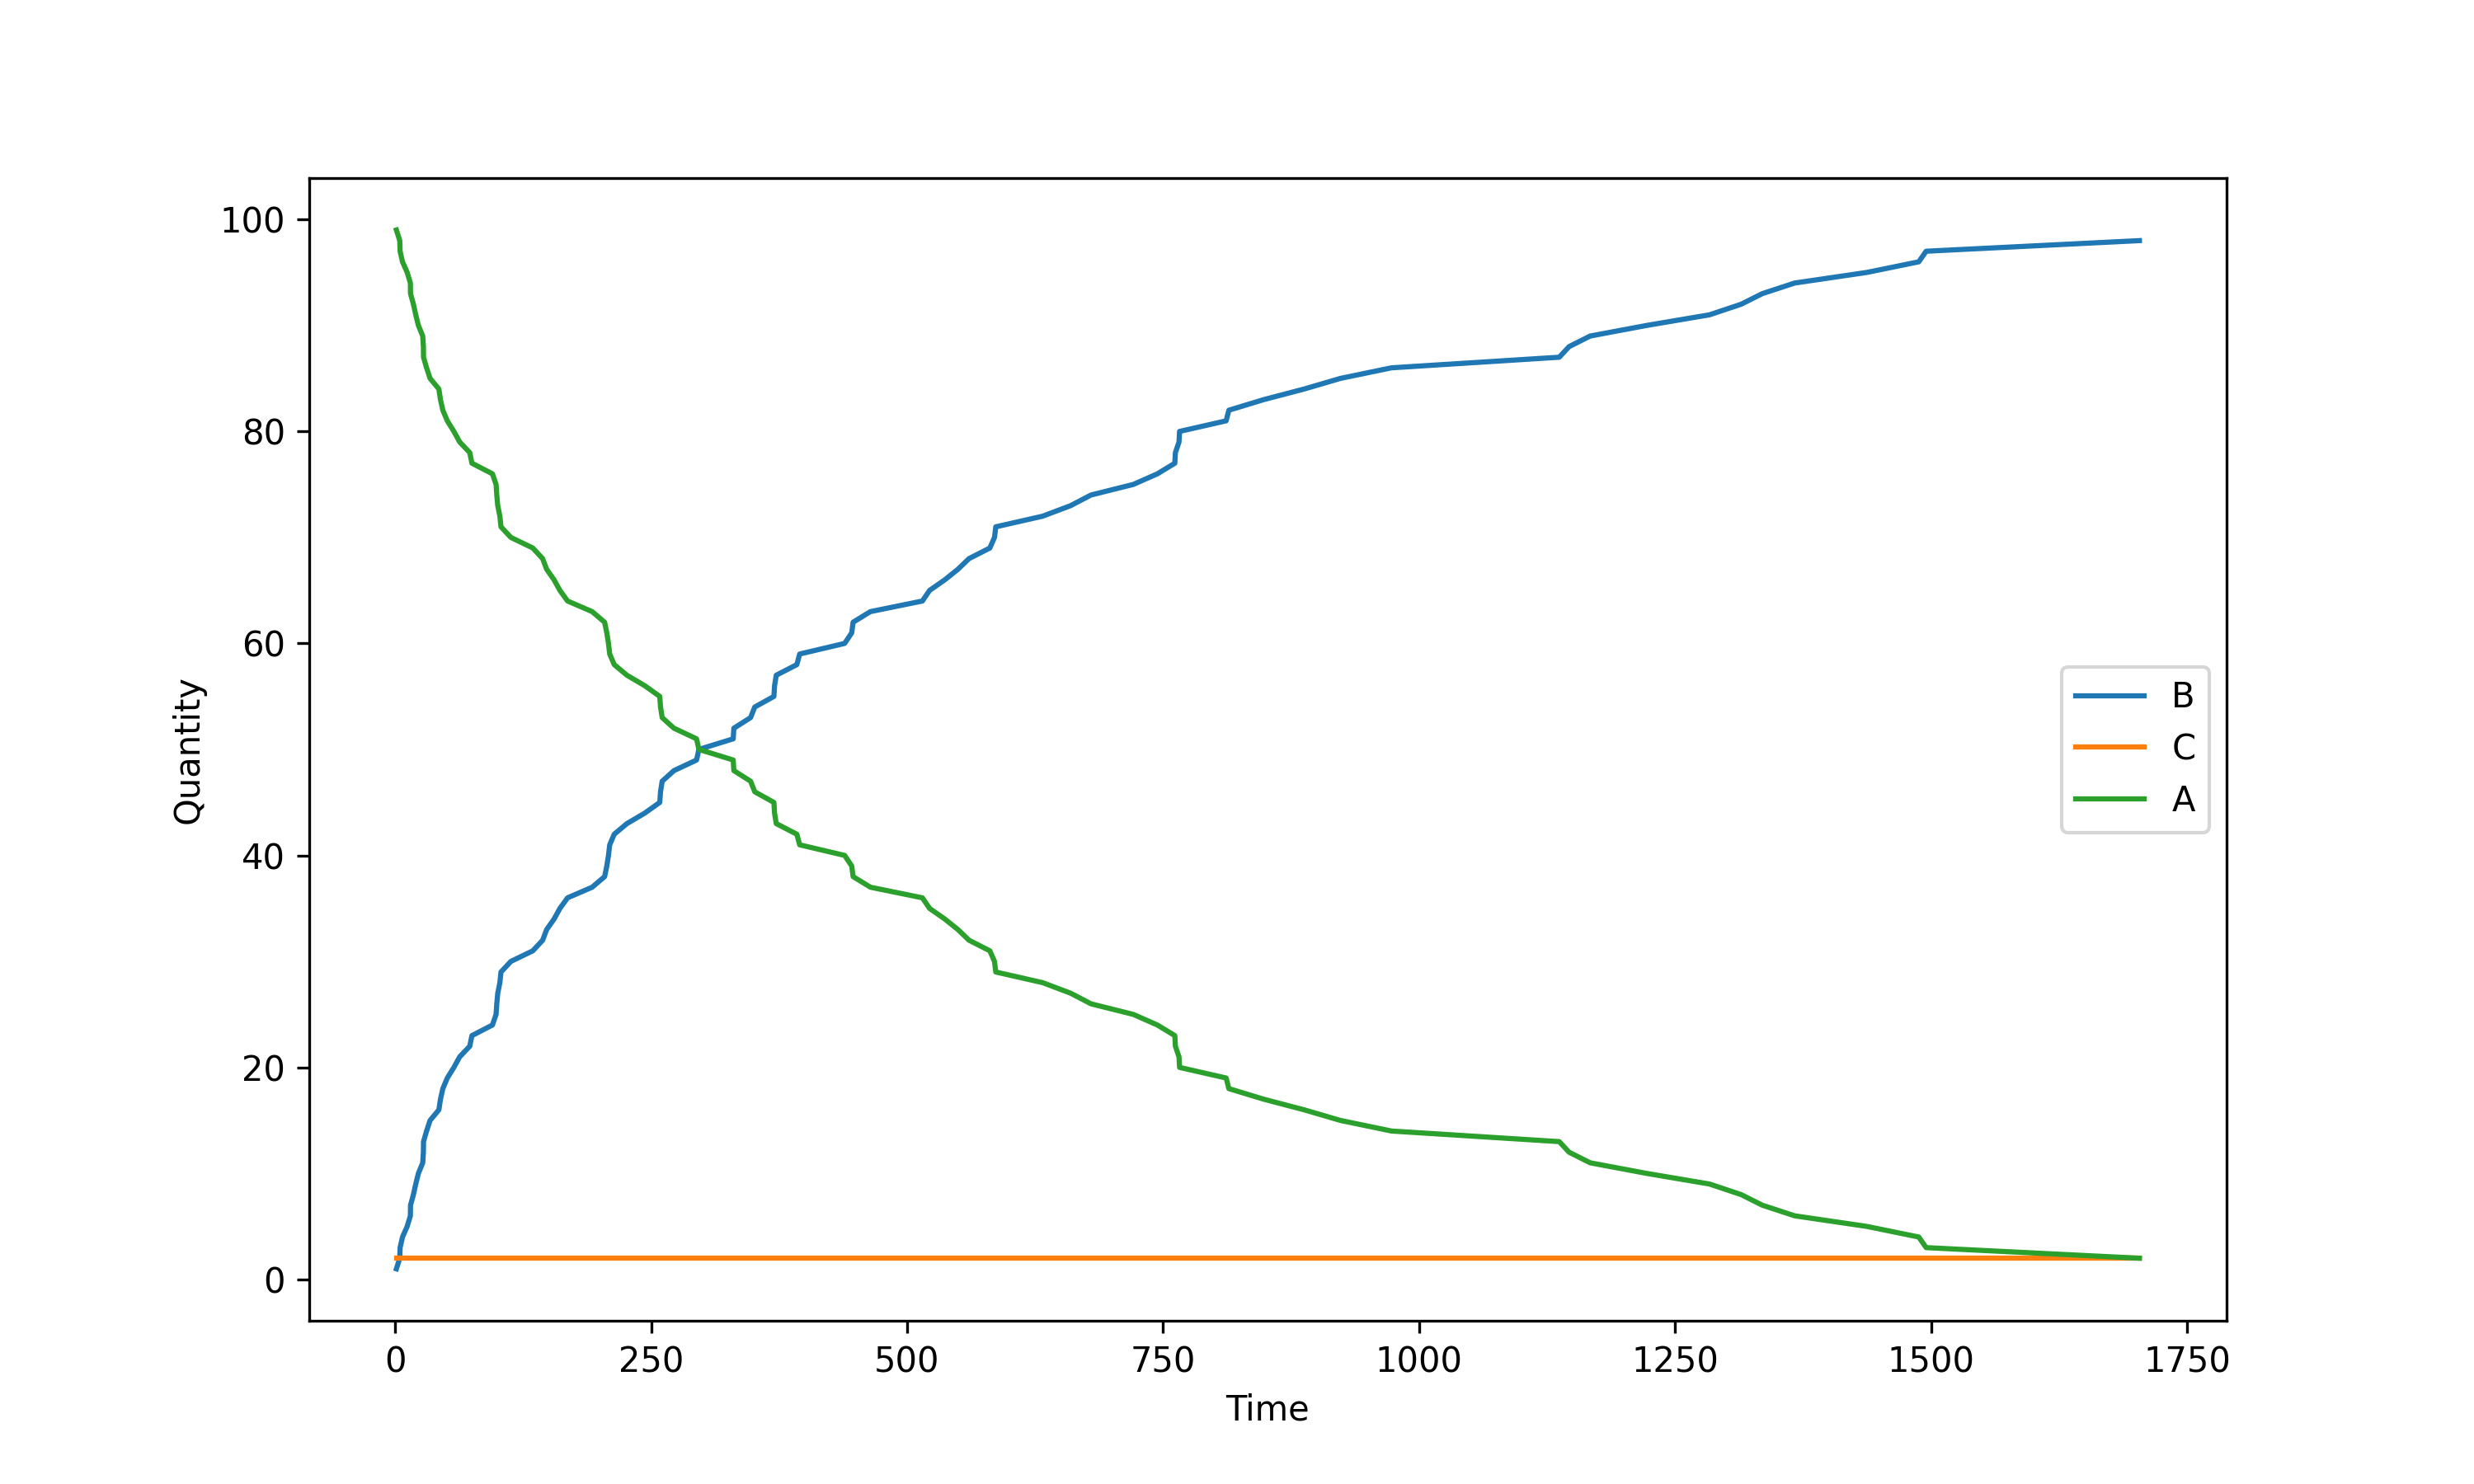
\includegraphics[width=\textwidth]{../plots/simple2}
	\caption{Plot of running the simple model simulation with A(0)=100, B(0)=0, C(0)=2.}
	\label{fig:plot_simple2}
\end{figure}

\begin{figure}[H]
	\centering
	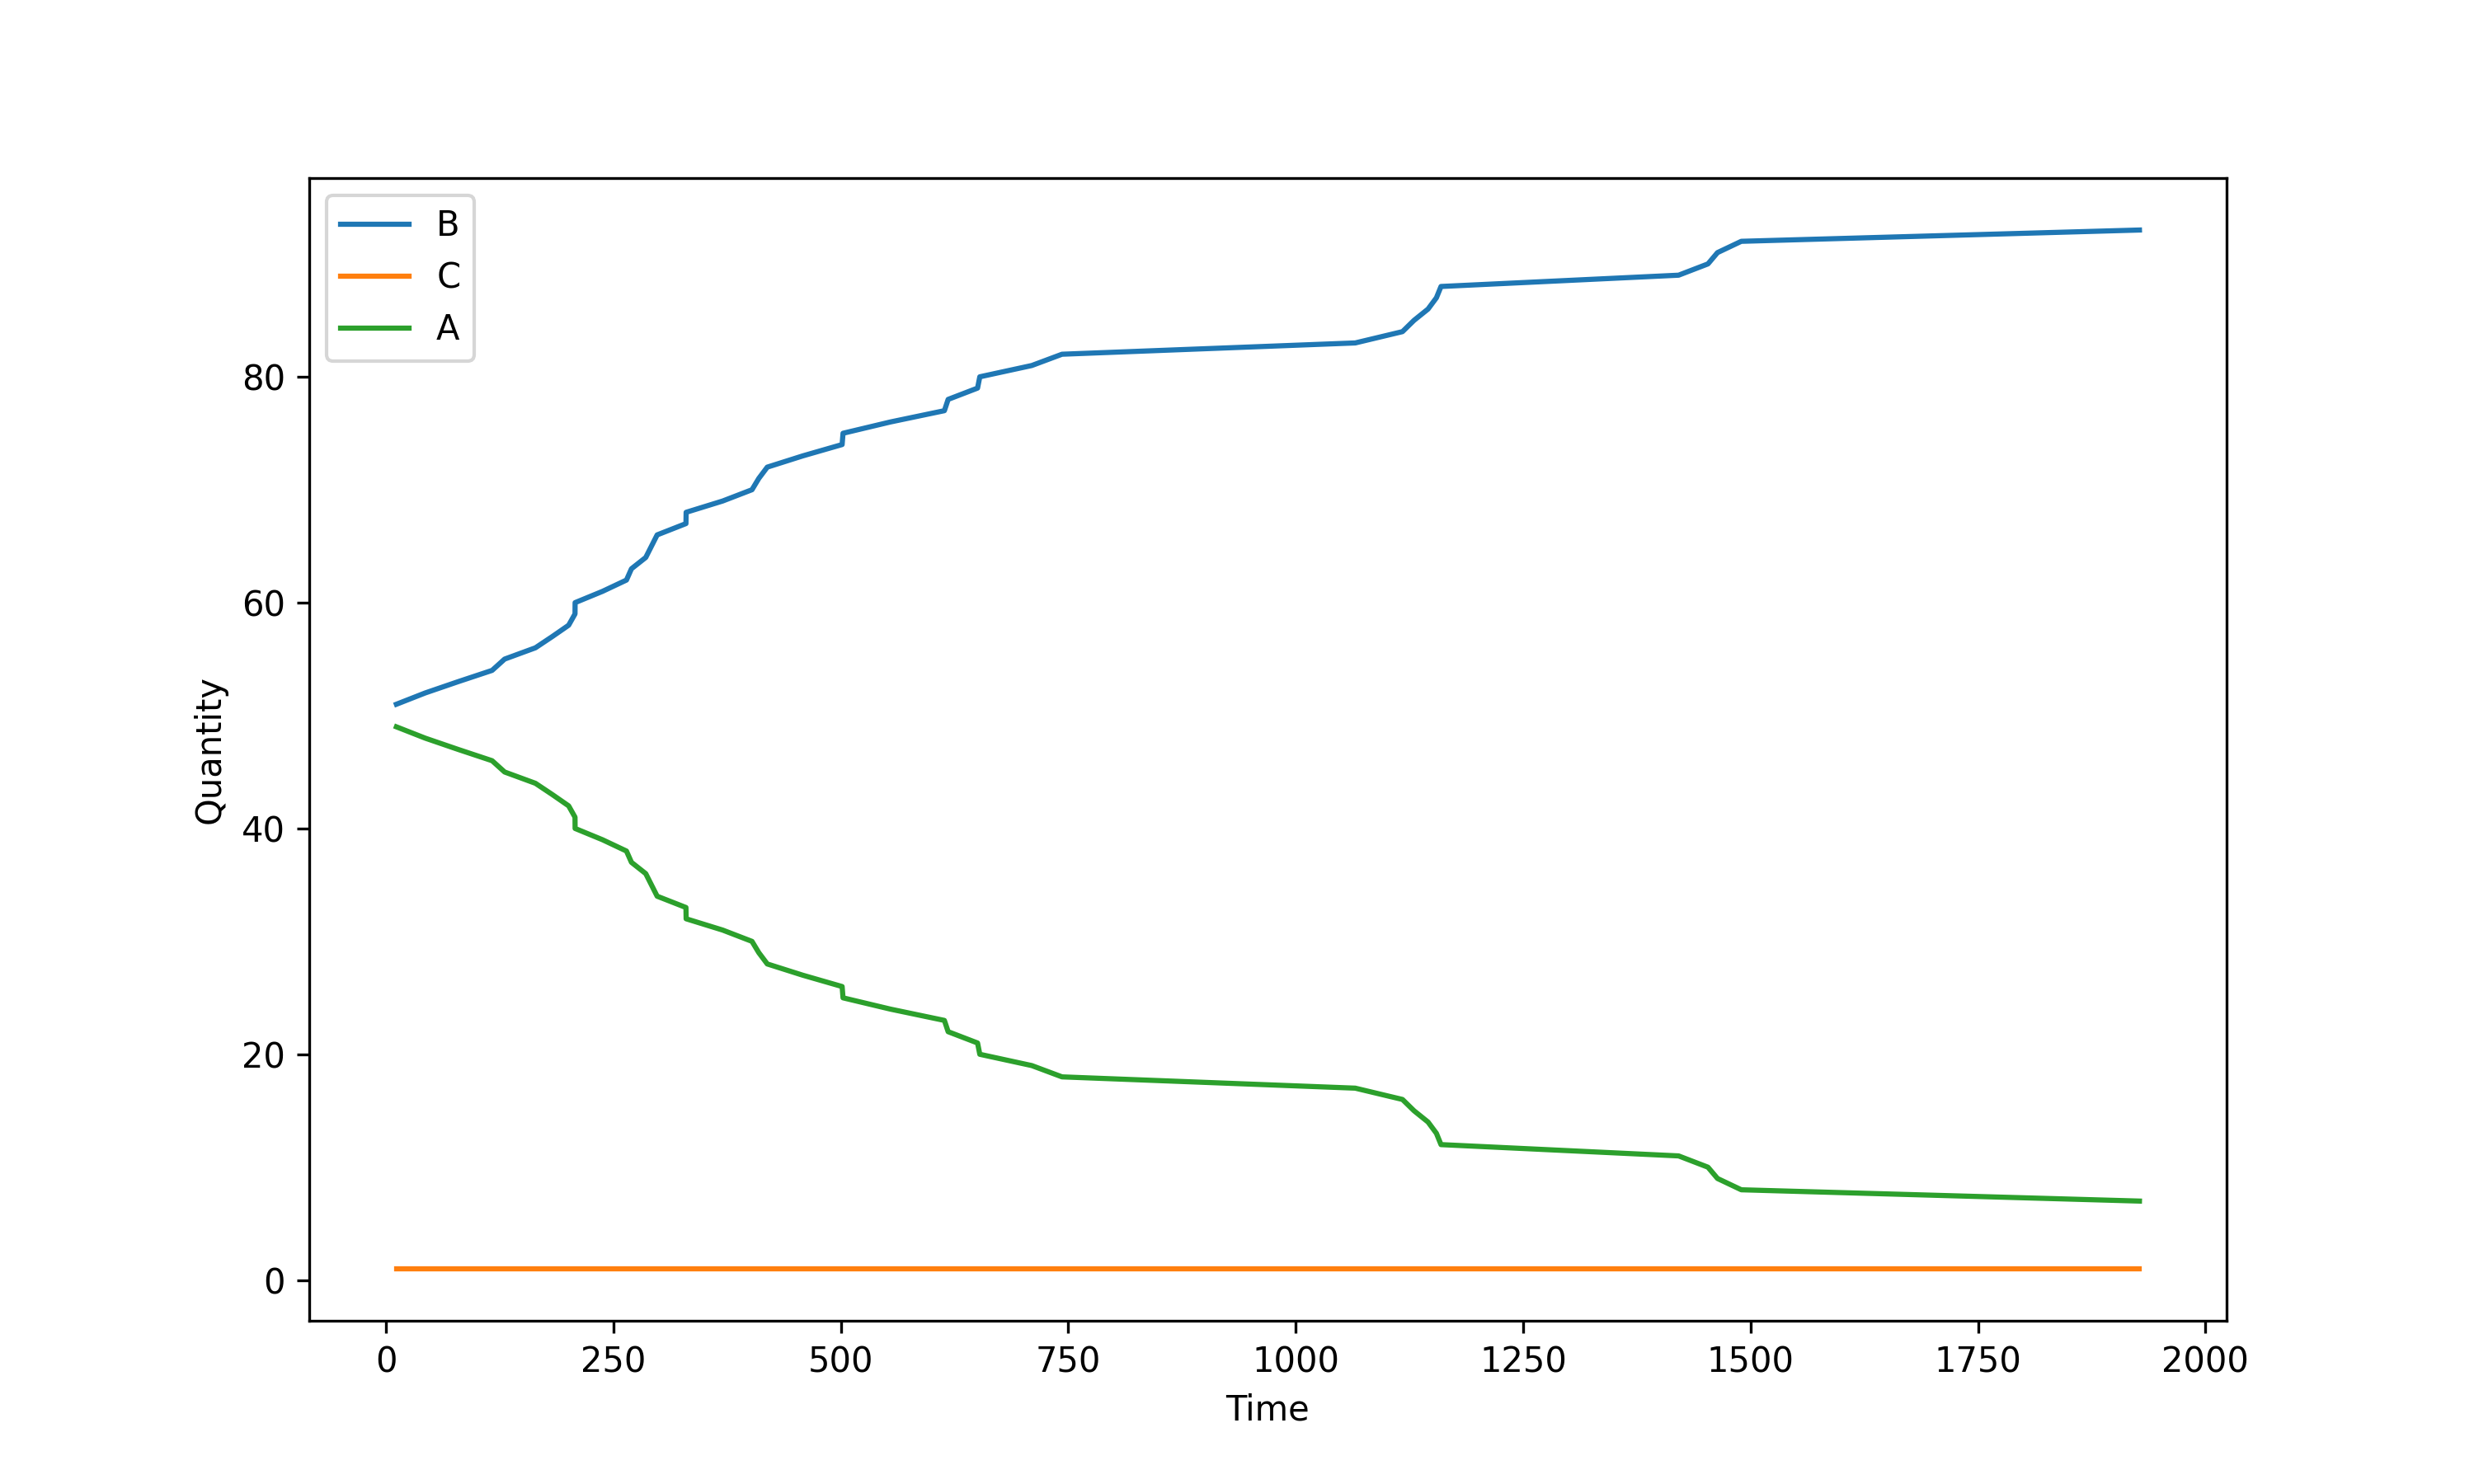
\includegraphics[width=\textwidth]{../plots/simple3}
	\caption{Plot of running the simple model simulation with A(0)=50, B(0)=50, C(0)=1.}
	\label{fig:plot_simple3}
\end{figure}

\begin{figure}[H]
	\centering
	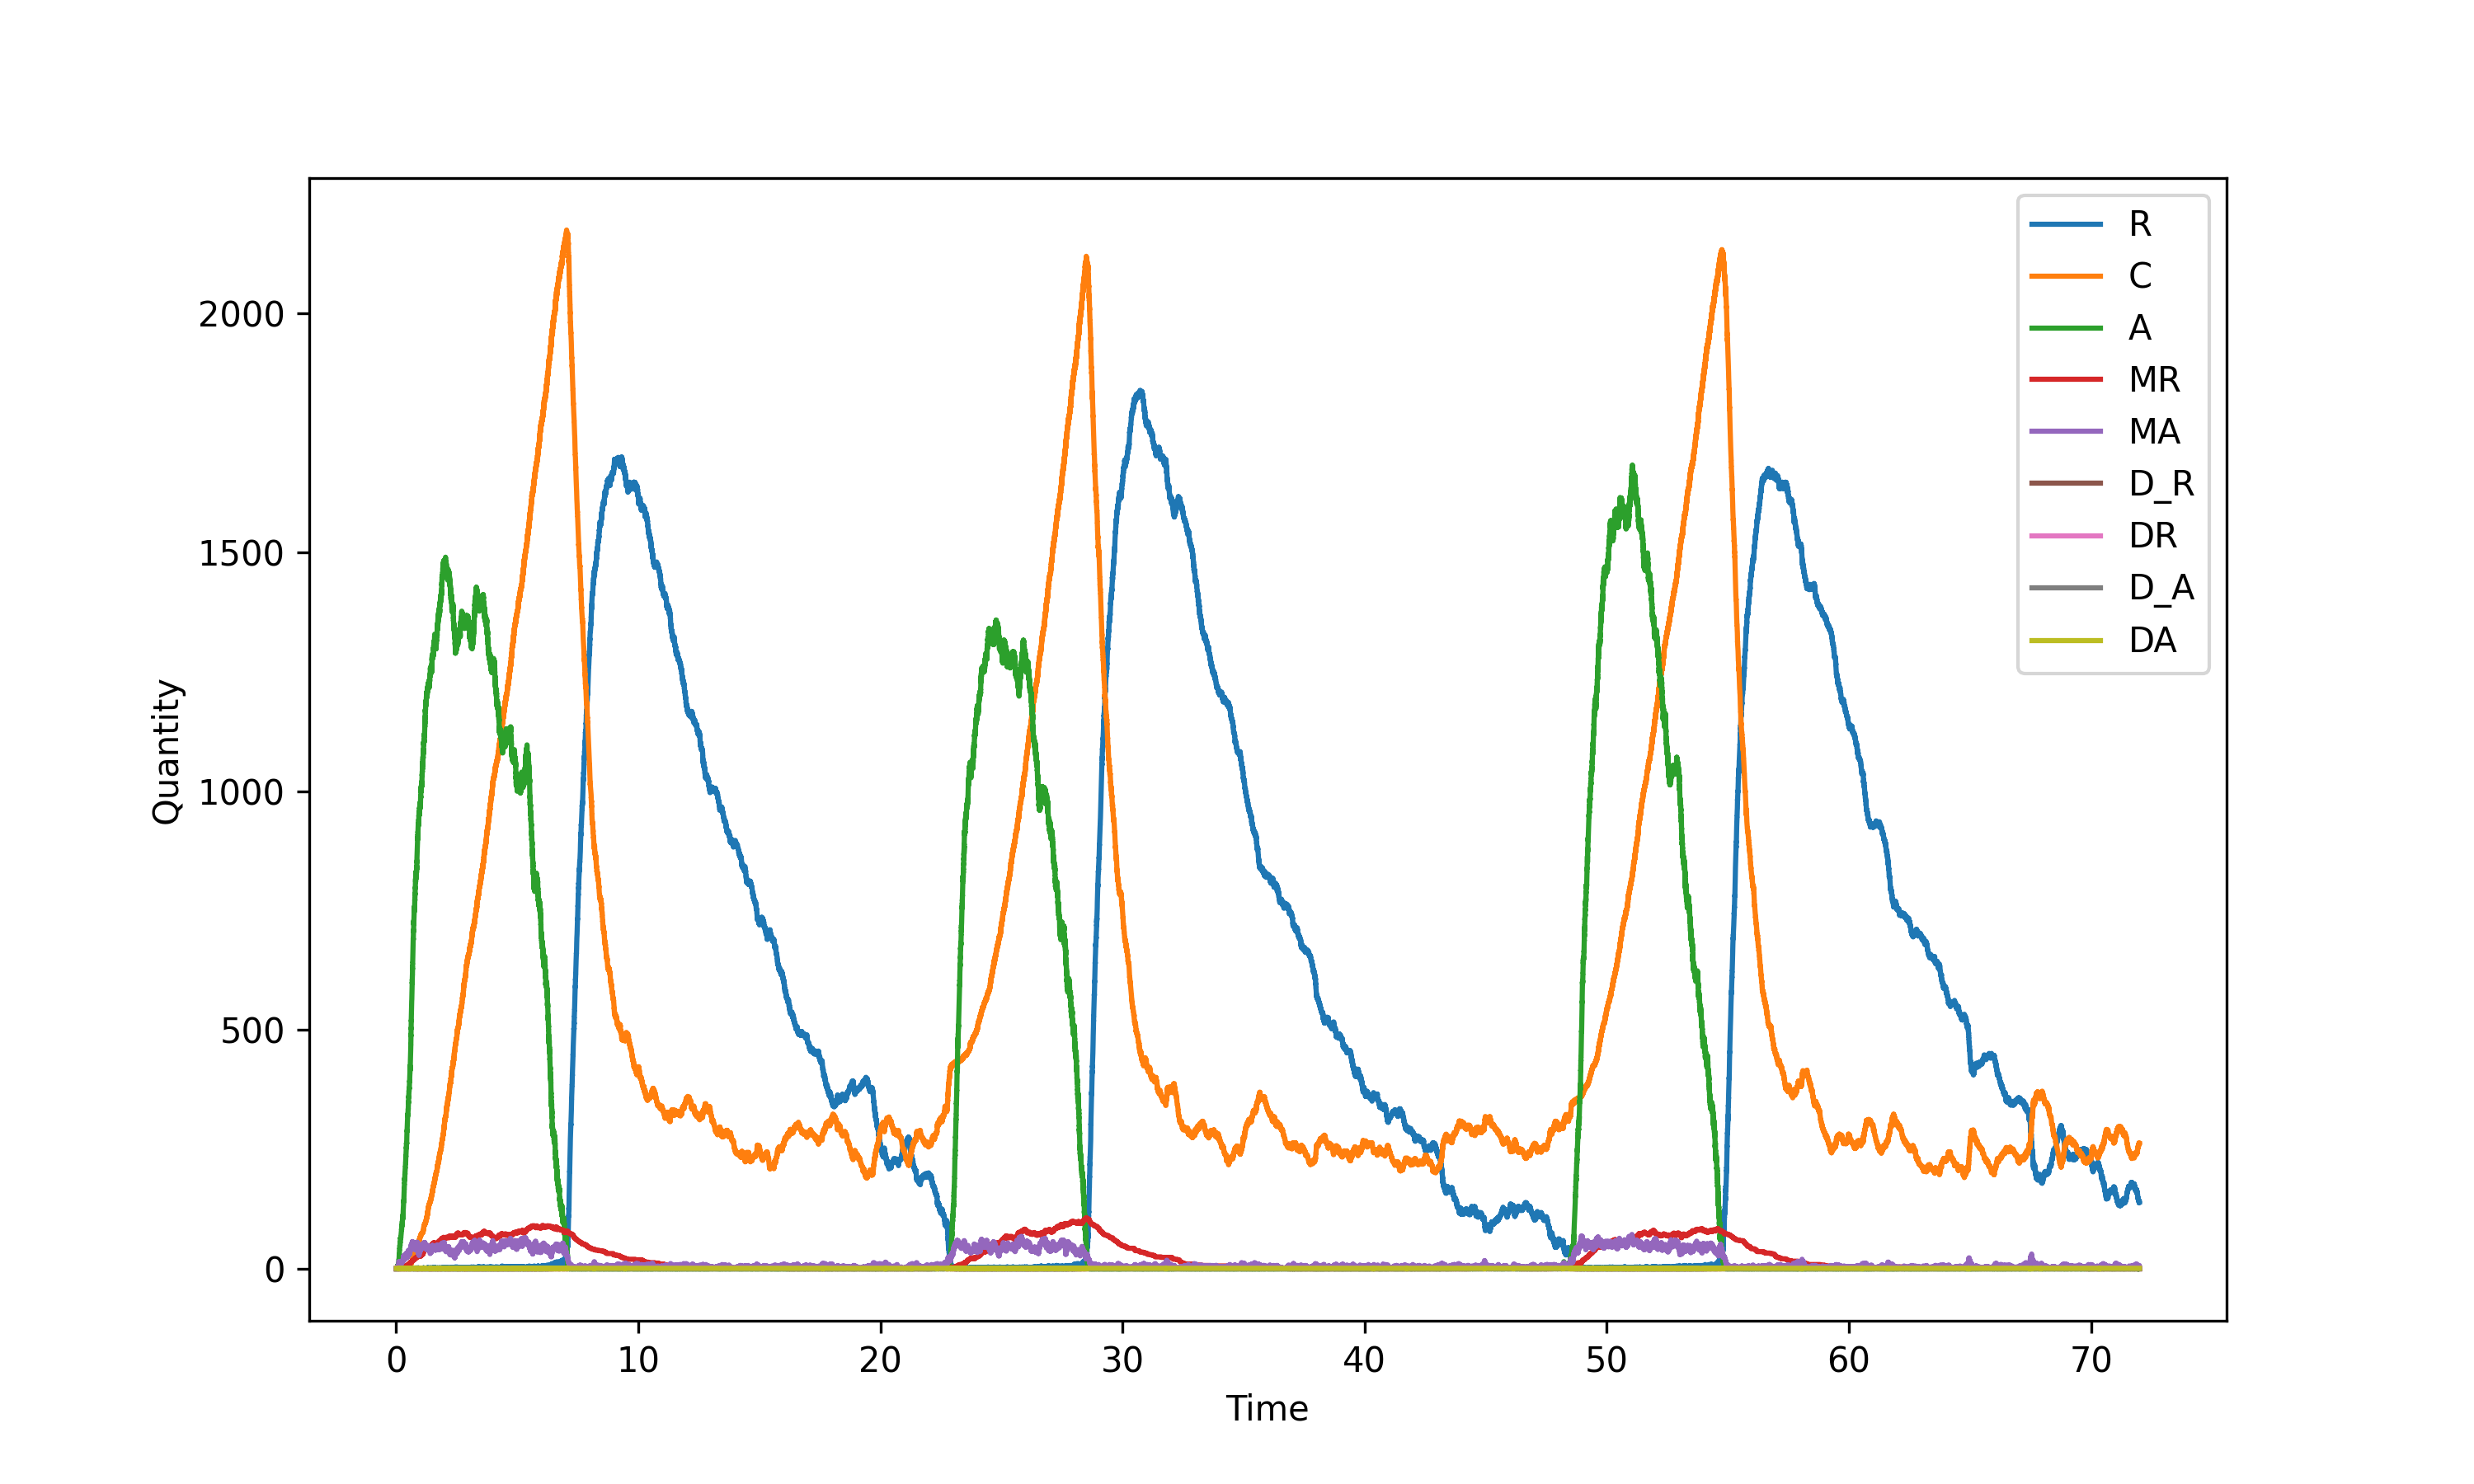
\includegraphics[width=\textwidth]{../plots/circadianOscillator.png}
	\caption{Plot of running the circadian oscillator model simulation.}
	\label{fig:plot_circadianOscillator}
\end{figure}

\begin{figure}[H]
	\centering
	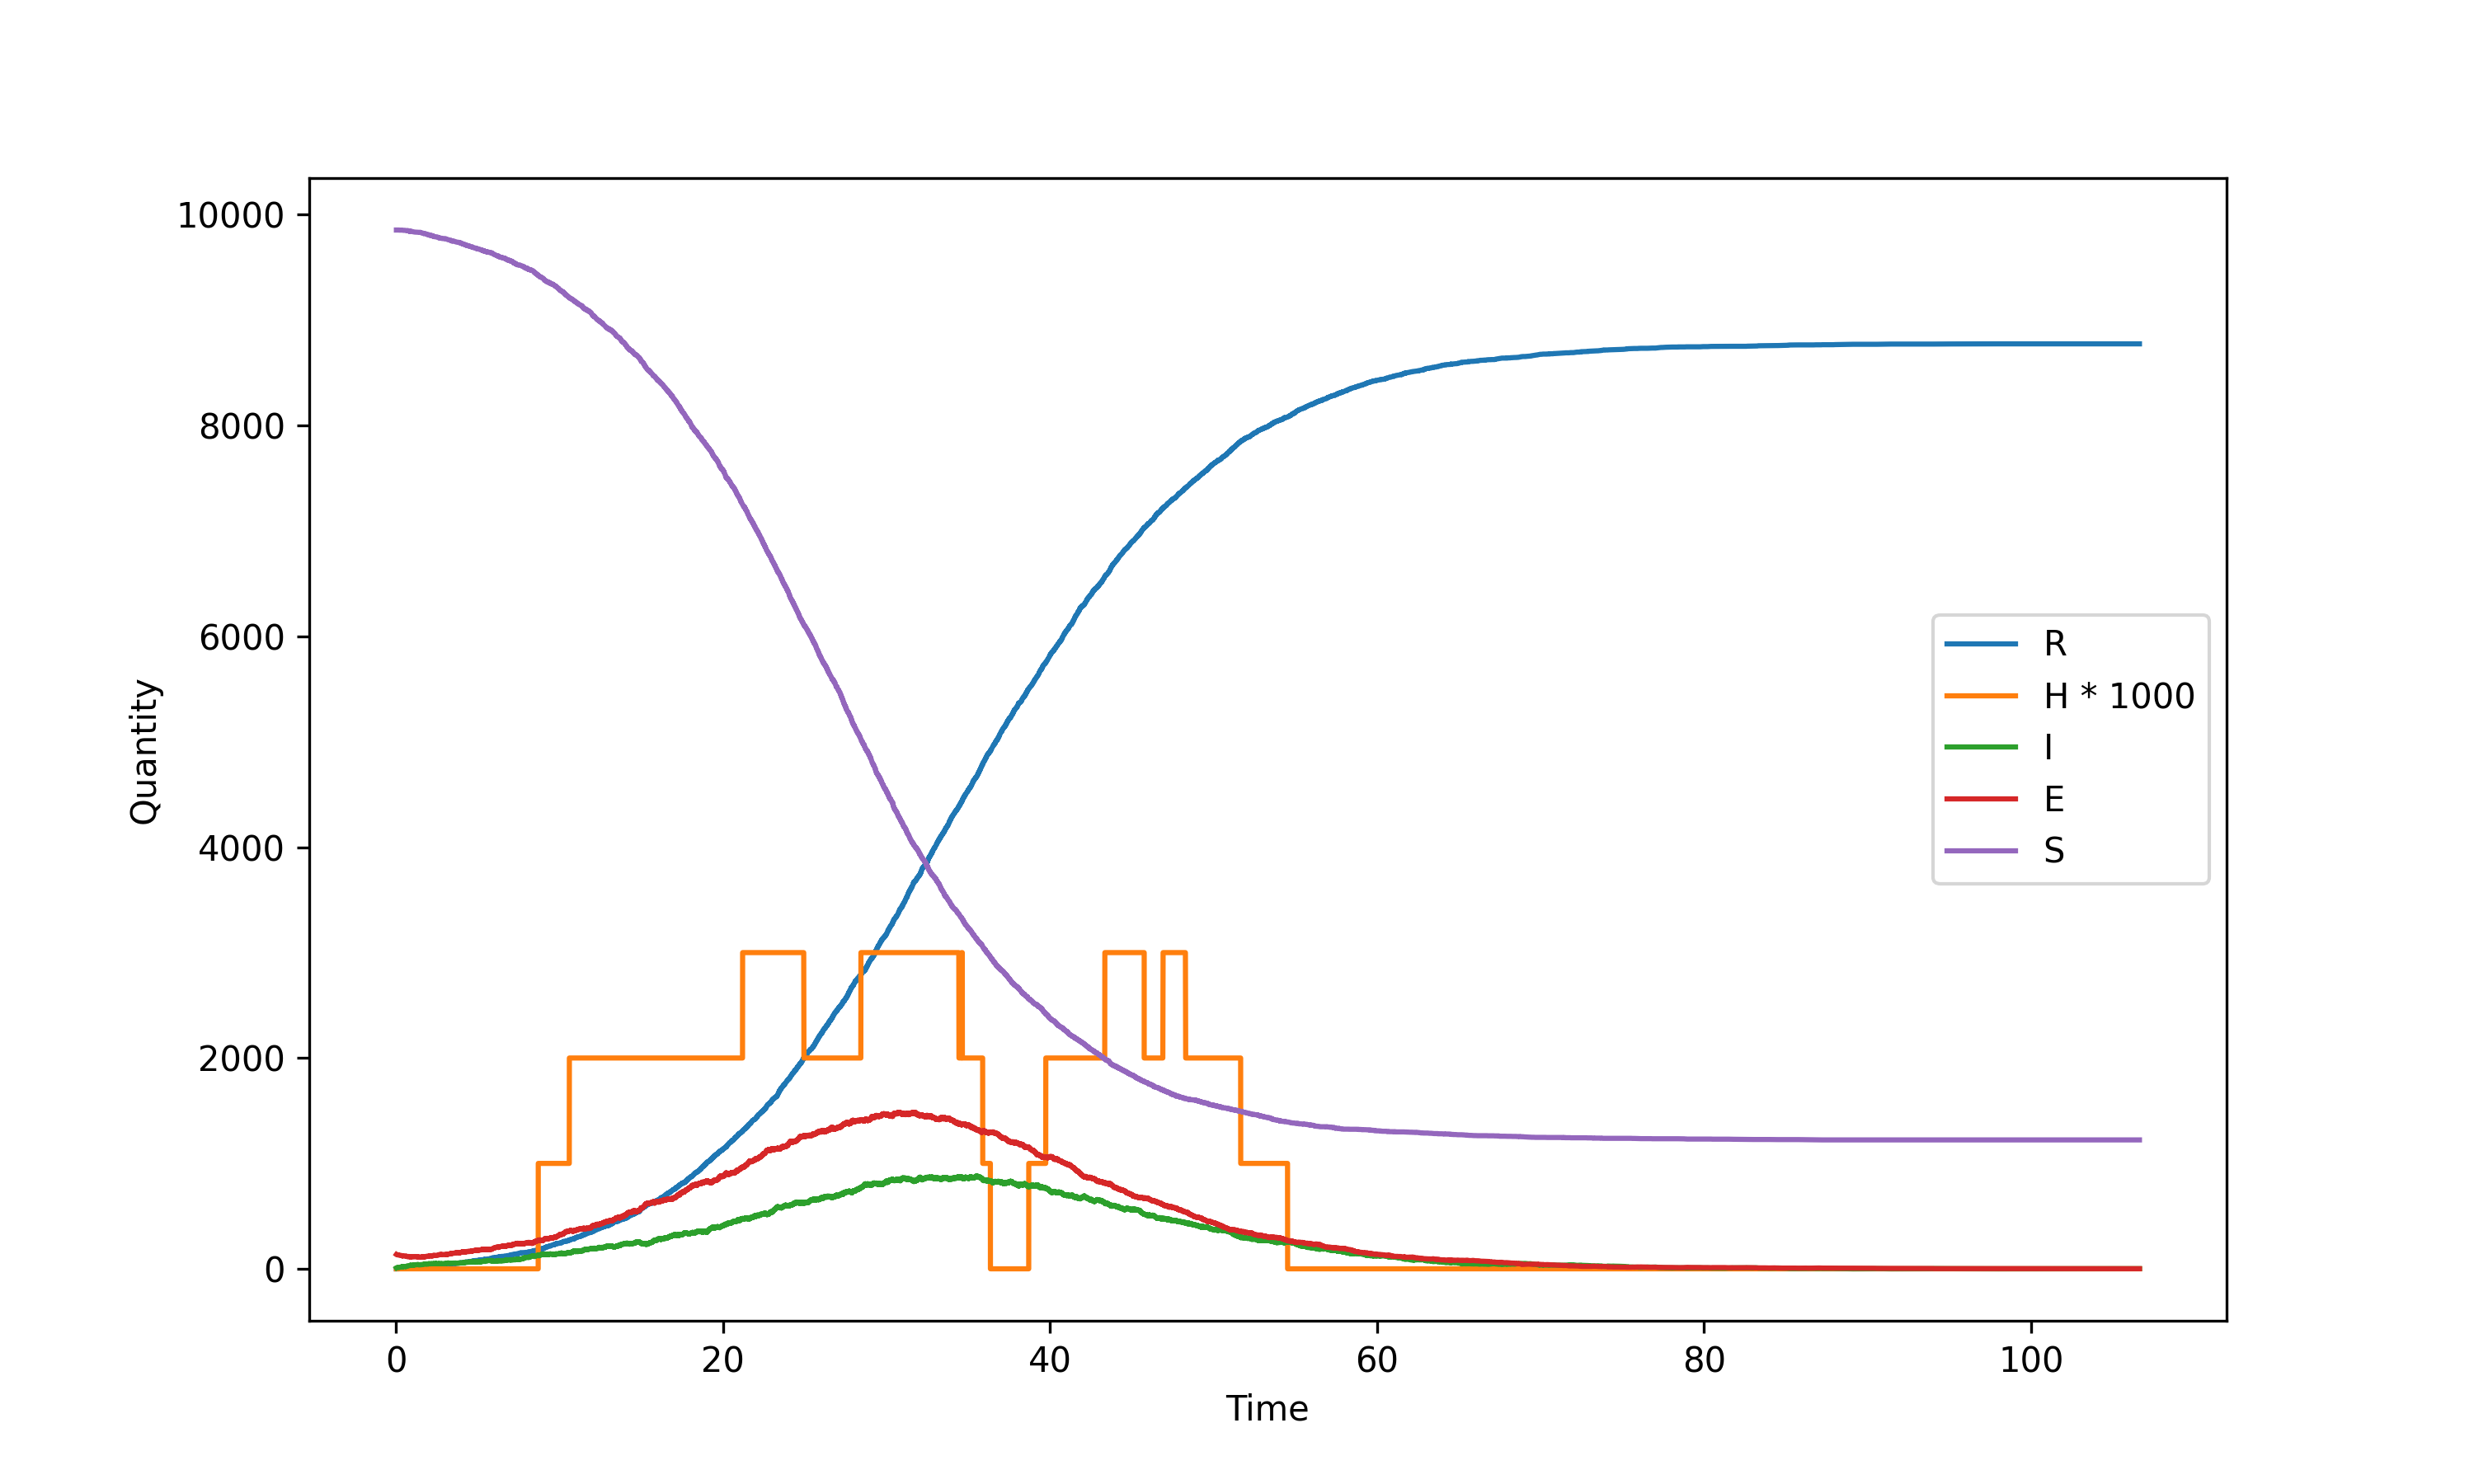
\includegraphics[width=\textwidth]{../plots/seihr.png}
	\caption{Plot of running the SEIHR model simulation.}
	\label{fig:plot_seihr}
\end{figure}

\subsection{Benchmarks}
\begin{figure}[H]
	\centering
	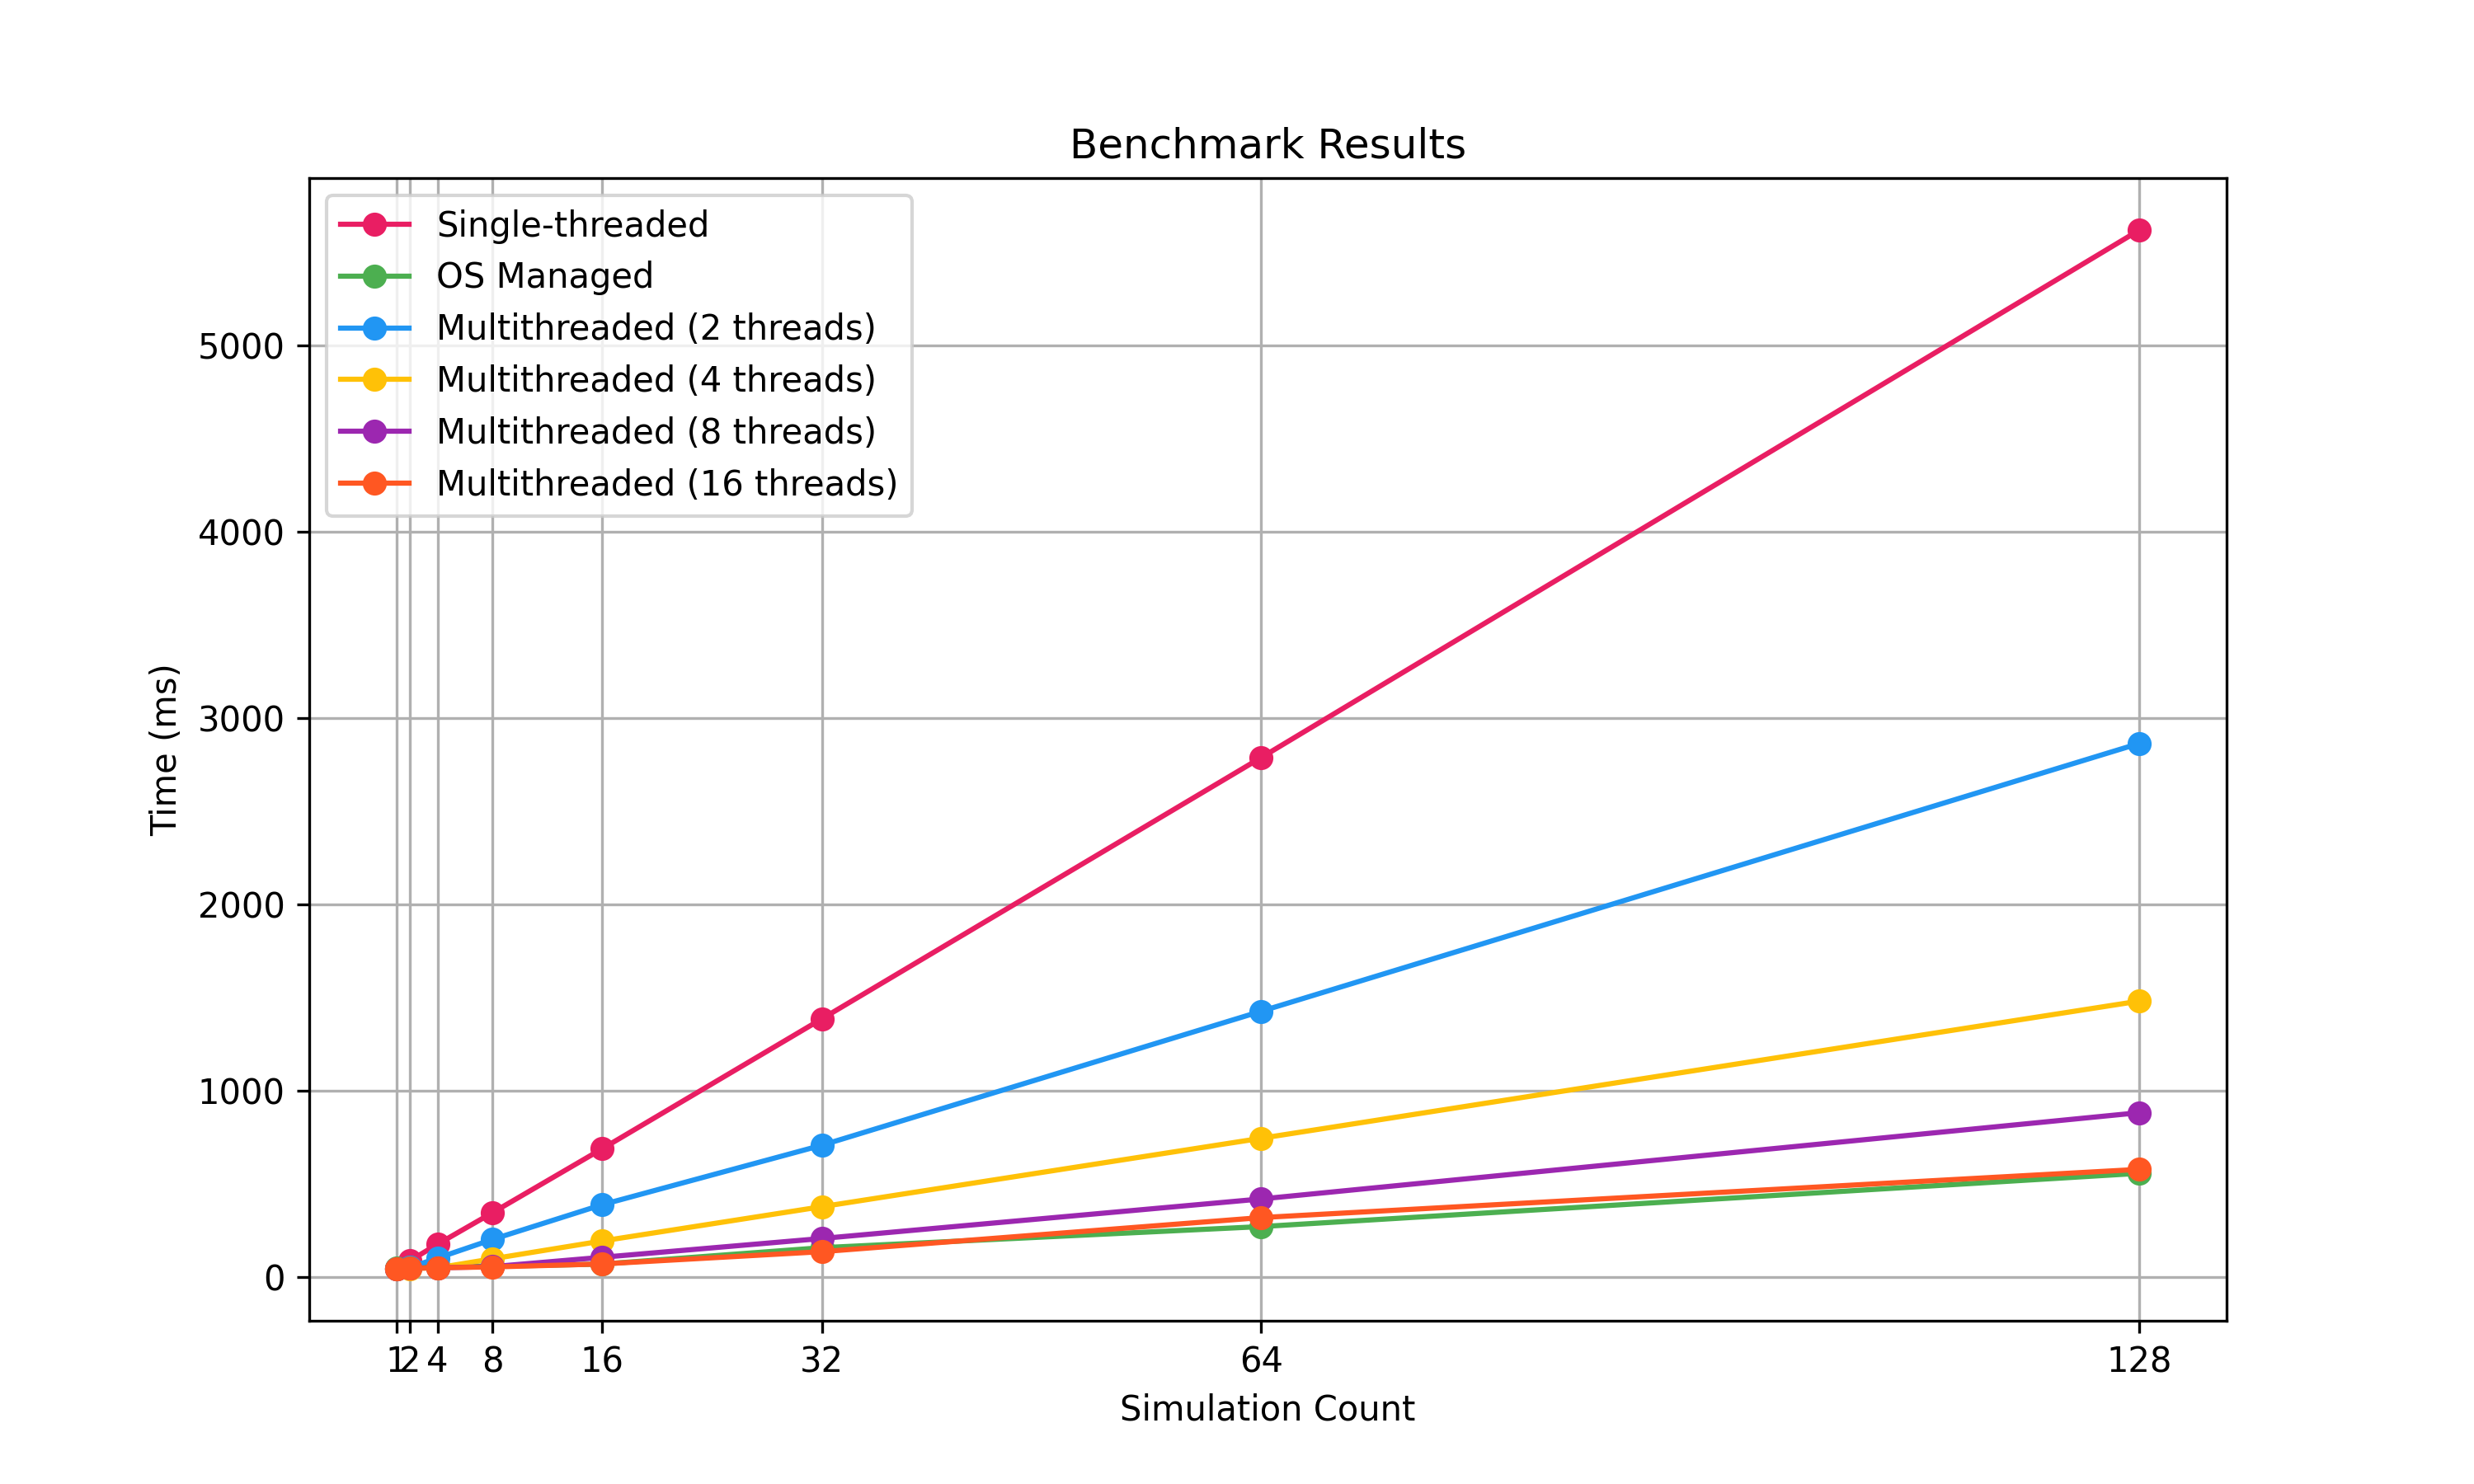
\includegraphics[width=\textwidth]{../benchmark/multithread_benchmark_with_sync.png}
	\caption{Benchmark of model simulation.}
	\label{fig:benchmark_multithread_with_sync}
\end{figure}

\begin{figure}[H]
	\centering
	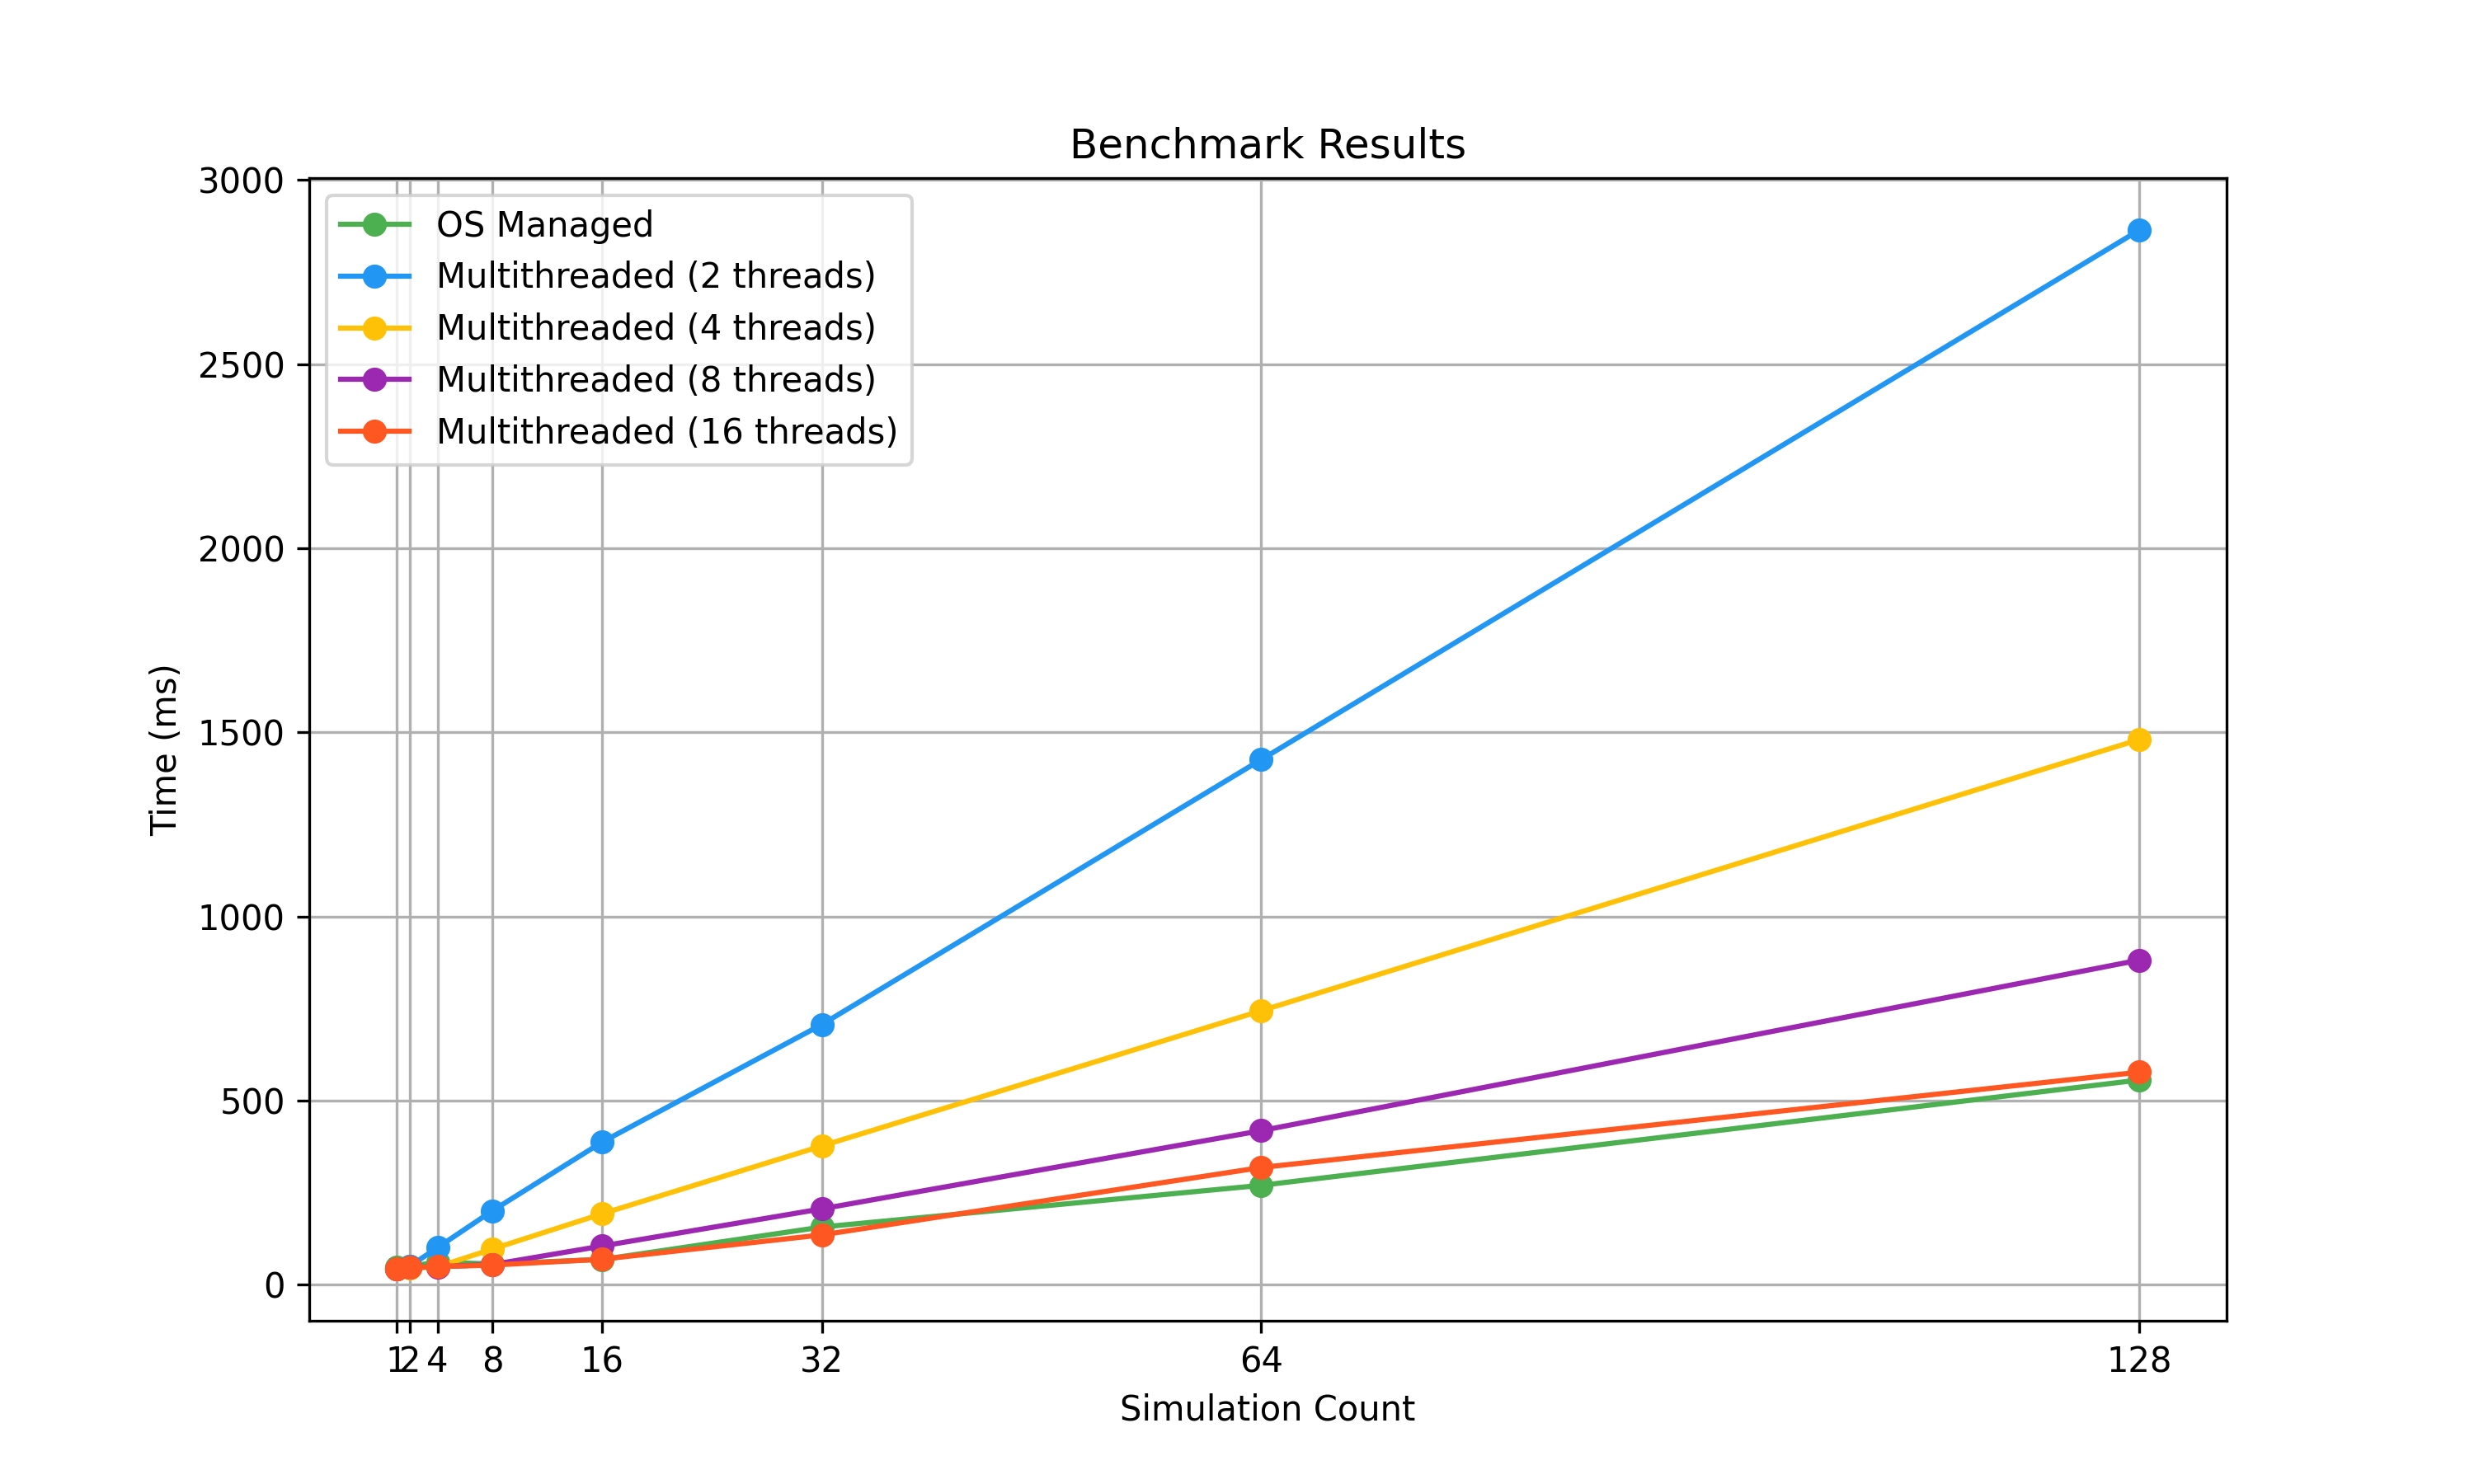
\includegraphics[width=\textwidth]{../benchmark/multithread_benchmark_without_sync.png}
	\caption{Benchmark of model simulation not including benchmarks for synchronized model simulation.}
	\label{fig:benchmark_multithread_without_sync}
\end{figure}